\subsection{Communications Overview}

What is it, why do we need it and a spec of sorts. Then explain the layered structure.


The aim of this project was to produce a general-purpose modular robotics platform - and any form of general-purpose modular robot requires some form of communications between modules. When designing the communication system for this project we had a number of specifications we wished to meet, summarized below:

\begin{itemize}
\item Reliable neighbor to neighbor data transmission between connected modules [High priority].
\item Modules should be able to communicate between modules connected to all six connection ports [High priority].
\item Modules should be capable of choosing which data is sent to which connection ports - i.e. they should be able to direct their data transmission and not just broadcast it [High priority].
\item Masterless operation should be possible - no module should need to be designated as a `master' node -  the system should work if all modules are identical [High priority].
\item Full duplex operation should be possible - modules should be able to send data as they are receiving [Medium priority].
\item Modules should be able to determine which connection port data is sent from, to enable inference of the physical structure of the modular robot system [Medium priority].
\item The communications system should be scalable with the number of connected robots and capable of supporting a reasonably large sized communications network [Medium priority].
\end{itemize}

%We also had a number of constraints by virtue of the technology available to us and our budget. Some were apparent initially and others were discovered after research. They are listed below:

%\begin{itemize}
%\item
%\end{itemize}

Below we describe the design of the communication system for this project. In order to simplify design, implementation and understanding of this system we split it up into a number of `layers' which build upon each other to create a working communication stack. We begin with the bottommost layer: the \emph{physical layer}, which is responsible for transmitting and receiving raw bytes to and from the connection ports, and contains the physical hardware used to do this. We then move on to the \emph{neighbor to neighbor packet layer}, building on the physical layer which handles reliable communications between connected devices. The next layer: the \emph{network layer} then builds directly on the neighbor to neighbor packet layer, and is responsible for transmitting packets across a network of connected modules. Finally the \emph{application layer} uses both the neighbor to neighbor and network layers, and is the layer responsible for utilizing the communications system and doing useful work.

\subsection{Physical Layer}

The physical layer has a simple responsibility: transmitting and receiving bytes of data to and from each of the six connection ports, according to the specification detailed above. 

The first step in designing the physical layer was choosing a bus technology to build it on. Initially I$^{2}$C was seen as a possible method for communication. The ATMega644P chip used to implement this project incorporates an I$^{2}$C controller, meaning implementing a bus would be trivial. 

However, although I$^{2}$C is specifically designed for communicating between a large number of connected components, implementing a masterless system with identical modules would not be easy. I$^{2}$C has a requirement that a single pair of pullup resistors be added to the bus. In order to fulfill this requirement and keep all modules identical pullups would need to be added to every device, which would affect scalability, since a large number of pullups on the line would degrade performance, and possibly stop the system working at all. Additionally, I$^{2}$C would not allow any form of inference of physical structure, since all devices are connected to a single bus. This means that there is no simple way of determining which connection port incoming messages are being received from, or indeed any way of sending messages specifically to one connection port and not others.

After much research and preliminary design work it was decided to use the simple UART (Universal Asynchronous Receiver/Transmitter)  serial ports on the ATMega644P for communication. Due to the reasonably unusual requirements of this project, i.e. the requirement that six modules be communicated with separately, it was not possible to find any suitable off-the-shelf solutions - for example, the ideal setup would be to use 6 USART ports - one for each of the connection ports - but no suitable hardware within our budget range existed to allow this.

Instead a multiplexer and decoder are used to connect the 6 connection ports to one serial port. A 3 bit control bus connected to both multiplexer and decoder selects the connection port to receive/transmit to/from, while the multiplexer then routes incoming data from the selected connection port to the microcontroller UART, ignoring the other connection port inputs. The decoder is used to selectively send data from the microcontroller UART to the selected connection port. In this way it is possible to send and receive data to and from different connection ports selectively. 

However, using this scheme alone it is impossible for the microcontroller to determine when data is being transmitted to it from a connection port that it is not currently requesting the multiplexer to route - the microcontroller does not know what port to listen to and when. Various methods for handling this problem were investigated, such as scanning over the connection ports one by one and listening for transmissions. Eventually however a more asynchronous scheme was designed: by connecting six pins on the microcontroller to the connection port receive lines it is possible for the microcontroller to `eavesdrop' on the incoming data and switch the multiplexer and decoder to the correct connection port when incoming data is detected.

Since each module may be connected to another module in two orientations (horizontally and vertically) it was decided that an additional 6 pins on the microcontroller be used to detect which orientation the module is connected in. By connecting the Rx wires for both orientations together and using a set of diodes to isolate the orientation detection pins from the horizontal Rx connection port wires it is possible to detect which orientation a module is connected - when connected in the vertical orientation the orientation detection pins will see no incoming data, but when connected horizontally these orientation pins will see the same signals as the eavesdropping pins.

HAVE FIGURE OF CIRCUIT WITH AREAS HIGHLIGHTED AND LABELED AND REFER TO THEM HERE.

SERIAL SPEC I.E. BAUD RATE, PARITY BITS, BITS PER BYTE THING etc

\subsection{Neighbor to Neighbor Packet Layer}

The neighbor to neighbor packet layer builds upon the physical layer to enable the reliable transmission and receiving of `packets' of data over the connection ports. This layer is implemented in software on-board the microcontroller - a state machine representation of the receive logic for this layer can be seen in figure \ref{fig:state-machine-packet-layer-rx} and the transmit logic in figure \ref{fig:state-machine-packet-layer-tx}.

\begin{figure}[h]
	\centering
	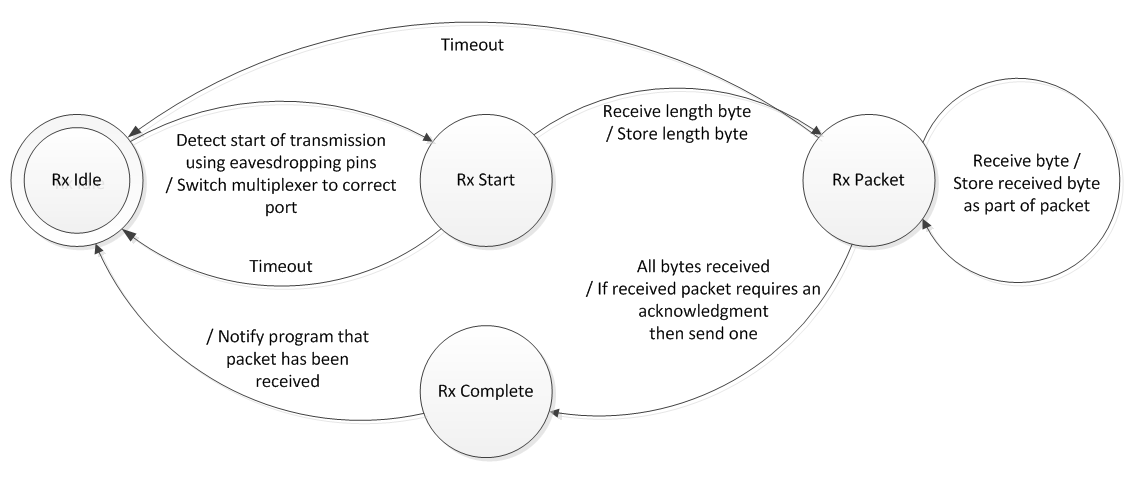
\includegraphics[width=1.0\textwidth]{Figures/state-machine-packet-layer-rx.png}
	\caption{State machine representation of the neighbor to neighbor packet layer receiving logic. Transition text is formatted as ``condition / action''.}
	\label{fig:state-machine-packet-layer-rx}    
\end{figure}

\begin{figure}[h]
	\centering
	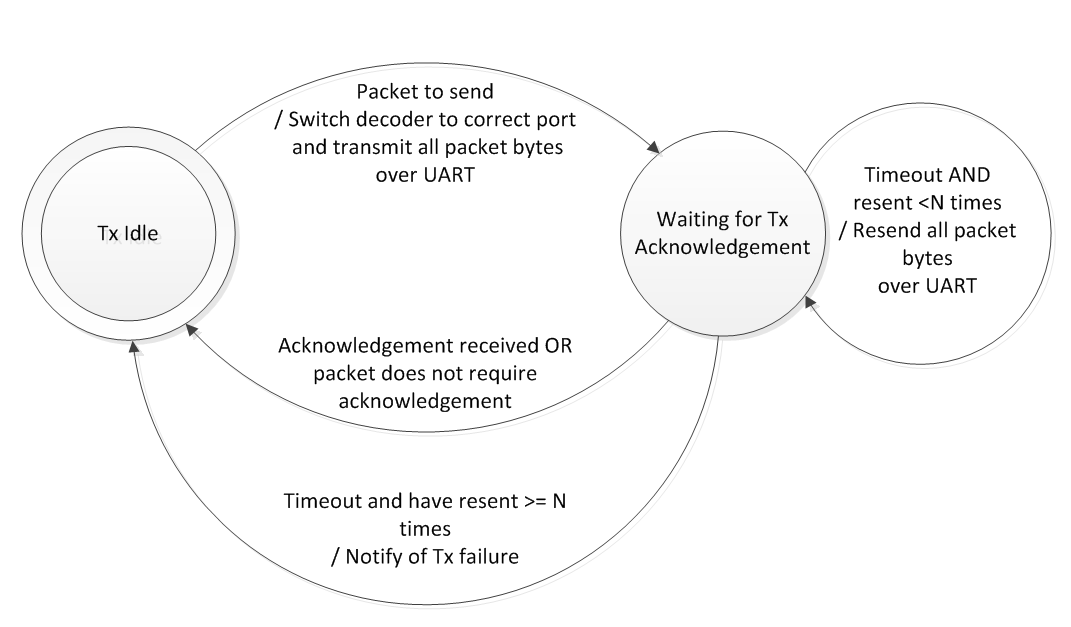
\includegraphics[width=0.7\textwidth]{Figures/state-machine-packet-layer-tx.png}
	\caption{State machine representation of the neighbor to neighbor packet layer transmitting logic. Transition text is formatted as ``condition / action''.}
	\label{fig:state-machine-packet-layer-tx}    
\end{figure}